\documentclass[tikz,crop]{standalone}

\usepackage{tikz}
\usetikzlibrary{positioning,backgrounds}

\begin{document}
    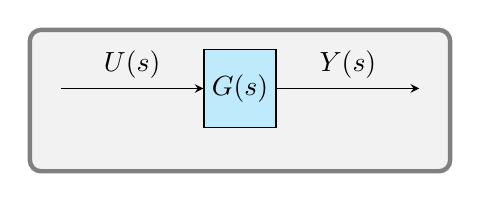
\begin{tikzpicture}[
        auto,
        >=stealth,
        node distance=12mm and 12mm,
        on grid,
        block/.style={draw, rectangle, minimum height=10mm, minimum width=6mm, inner sep=1mm},
        show background rectangle,
        background rectangle/.style={fill=gray!10, rounded corners, ultra thick,draw=gray},
    ]
        \node (input) at (0,0) {};
        \node [block, right=24mm of input, fill=cyan!25] (plant) {$G(s)$};
        \node [right=24mm of plant] (output) {};

        \draw [->] (input) -- node[above]{$U(s)$} (plant);
        \draw [->] (plant) -- node[above, name=out]{$Y(s)$} (output);

        % dummy node to match the closed loop bounding box
        \node [below=12mm of out, inner sep=0mm, minimum size=0] {};
    \end{tikzpicture}
\end{document}
